\documentclass{article}%
\usepackage[T1]{fontenc}%
\usepackage[utf8]{inputenc}%
\usepackage{lmodern}%
\usepackage{textcomp}%
\usepackage{lastpage}%
\usepackage[head=40pt,margin=0.5in,bottom=0.6in]{geometry}%
\usepackage{graphicx}%
%
\title{\textbf{Lionel Messi volvió a ser convocado por la selección de Argentina}}%
\author{EFE}%
\date{07/03/2019}%
%
\begin{document}%
\normalsize%
\maketitle%
\textbf{URL: }%
http://www.el{-}nacional.com/noticias/futbol/lionel{-}messi{-}volvio{-}ser{-}convocado{-}por{-}seleccion{-}argentina\_273742\newline%
%
\textbf{Periodico: }%
EN, %
ID: %
273742, %
Seccion: %
Fútbol\newline%
%
\textbf{Palabras Claves: }%
Argentina, Fútbol, Lionel Messi\newline%
%
\textbf{Derecho: }%
2.1%
, Otros Derechos: %
\newline%
%
\textbf{\textit{El astro argentino no juega con el equipo absoluto desde la eliminación de la celeste en los octavos de final del Mundial de Rusia ante Argentina}}%
\newline%
\newline%
%
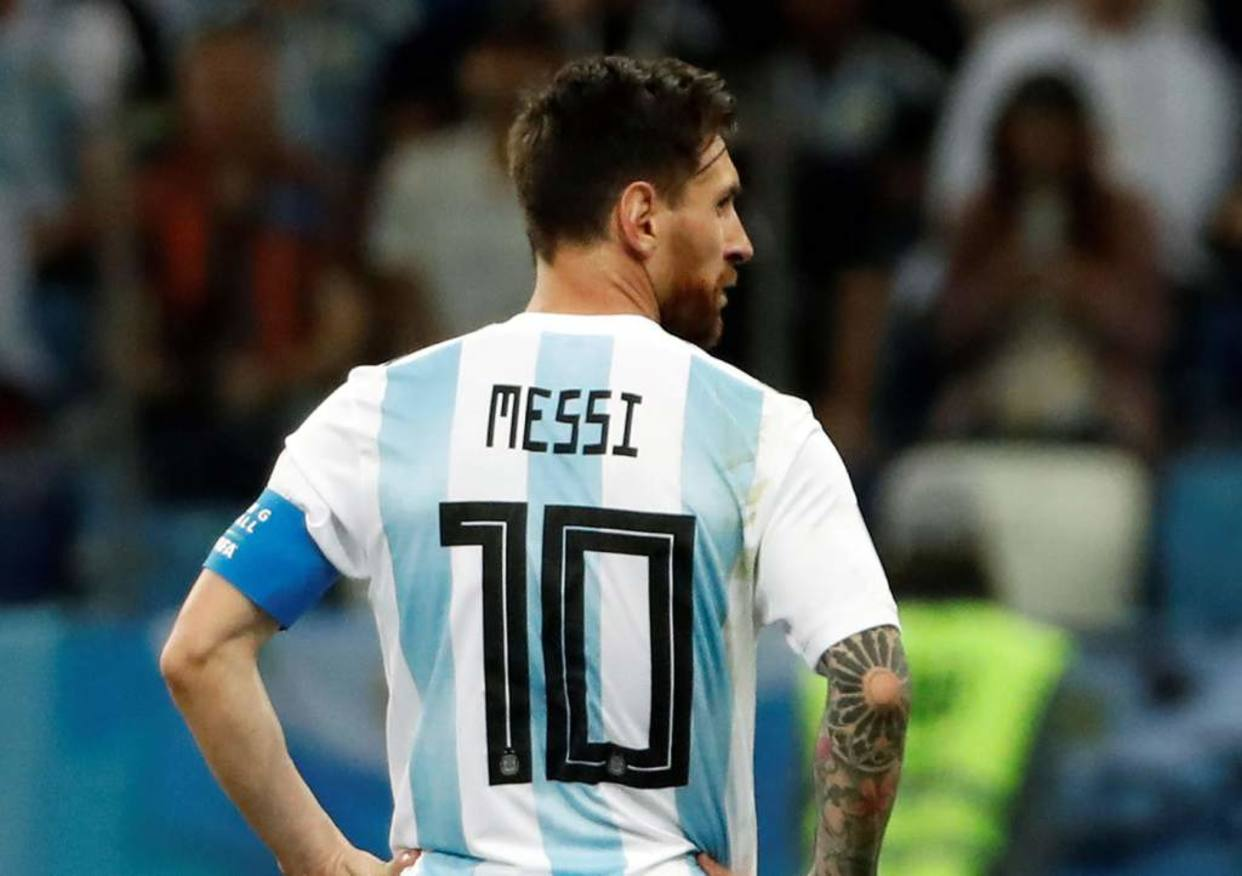
\includegraphics[width=300px]{EN_273742.jpg}%
\newline%
%
El futbolista argentino Lionel Messi se encuentra en la lista de jugadores convocados por la selección Argentina para los partidos amistosos ante Venezuela y Marruecos en la próxima fecha FIFA.%
\newline%
%
Messi~participó por última vez con la camiseta argentina el pasado 30 de junio, cuando su selección fue eliminada por Francia (4{-}3) en los octavos de final del Mundial de Rusia 2018.%
\newline%
%
En los últimos meses, tanto las autoridades de la Asociación del Fútbol Argentino~(AFA(, como el director técnico Lionel~Scaloni habían mostrado su deseo de que~Messi~retornara a la Albiceleste.%
\newline%
%
Entre las nuevas presencias destacan el delantero de River Plate Matías Suárez y el volante Domingo Blanco y el defensa Lisandro Martínez, de Defensa y Justicia y también destacan~las ausencias de Mauro Icardi, Sergio Agüero y Sergio Romero.%
\newline%
%
\end{document}